\documentclass{beamer}

\usetheme{Hannover}
%\usetheme{Montpellier}
%\usetheme{Pittsburgh}
%\usetheme{Warsaw}

\setbeamercolor{normal text}{fg=black}
\setbeamercolor{alerted text}{fg=black}
\setbeamercolor{structure}{fg=black}
\setbeamercolor{title}{fg=black}
\setbeamercolor{subtitle}{fg=black}
\setbeamercolor{section in toc}{fg=black}
\setbeamercolor{subsection in toc}{fg=black}
\setbeamercolor{frametitle}{fg=black}
\setbeamercolor{block title}{fg=black}
\setbeamercolor{block title alerted}{fg=black}
\setbeamercolor{block title example}{fg=black}
\setbeamercolor{section number projected}{bg=white,fg=black}

\setbeamertemplate{frametitle}[default][center]

\usepackage{graphicx} % for including graphics

%\usecolortheme{default}

\title[Union Organizing]{Construction Union Agreements\\
Union Organizing in Historical-Comparative Perspective}
\author{Matthew Carson}
\date[Undergraduate Research Week '24]{Undergraduate Research Week 2024}

\begin{document}

\begin{frame}
  \titlepage
\end{frame}

\begin{frame}{Table of Contents}
  \tableofcontents
\end{frame}

\section{Methods}
\begin{frame}{Methods}
\begin{columns}
	\column{0.3\textwidth}
	\newline
		\begin{minipage}[t][0.25\textheight][t]{\linewidth}
			Historical\\
			Within-Case\\
			Analyses
		\end{minipage}
		\vfill
		\begin{minipage}[b][0.4\textheight][b]{\linewidth}
			Comparative\\
			Between-Case\\
			Analyses
		\end{minipage}
	\column{0.7\textwidth}
	\newline
		\begin{minipage}[t][0.25\textheight][t]{\linewidth}
			\begin{itemize}
				\item Historical trajectory of the union.
				\item Durability: institutional arrangements.
				\item Structural features \& constraints.
				\item Institutional changes (mergers, etc.).
				\item Evolutionary or generative approach (Reed 1997).
			\end{itemize}
		\end{minipage}
		\vfill
		\begin{minipage}[b][0.4\textheight][b]{\linewidth}
			\begin{itemize}
				\item Differences in institutional features.
				\item Difference in political outcomes.
			\end{itemize}
		\end{minipage}
		\newline
		\newline
\end{columns}
\end{frame}




\subsection{Union Organizing Paths}
\begin{frame}{Union Organizing Paths}
  \begin{columns}
    \column{0.725\textwidth}
    \includegraphics[width=\linewidth]{../images/organizing_paths}

    \column{0.3\textwidth}
    The industrial mode of organizing (left) and the construction mode of organizing (right). Construction unions may follow either path, but other unions may not voluntarily negotiate the way that construction unions can.
    \end{columns}
\end{frame}

\section{Union Leverage}
\begin{frame} % {Union Leverage}
  \begin{columns}
    \column{0.725\textwidth}
    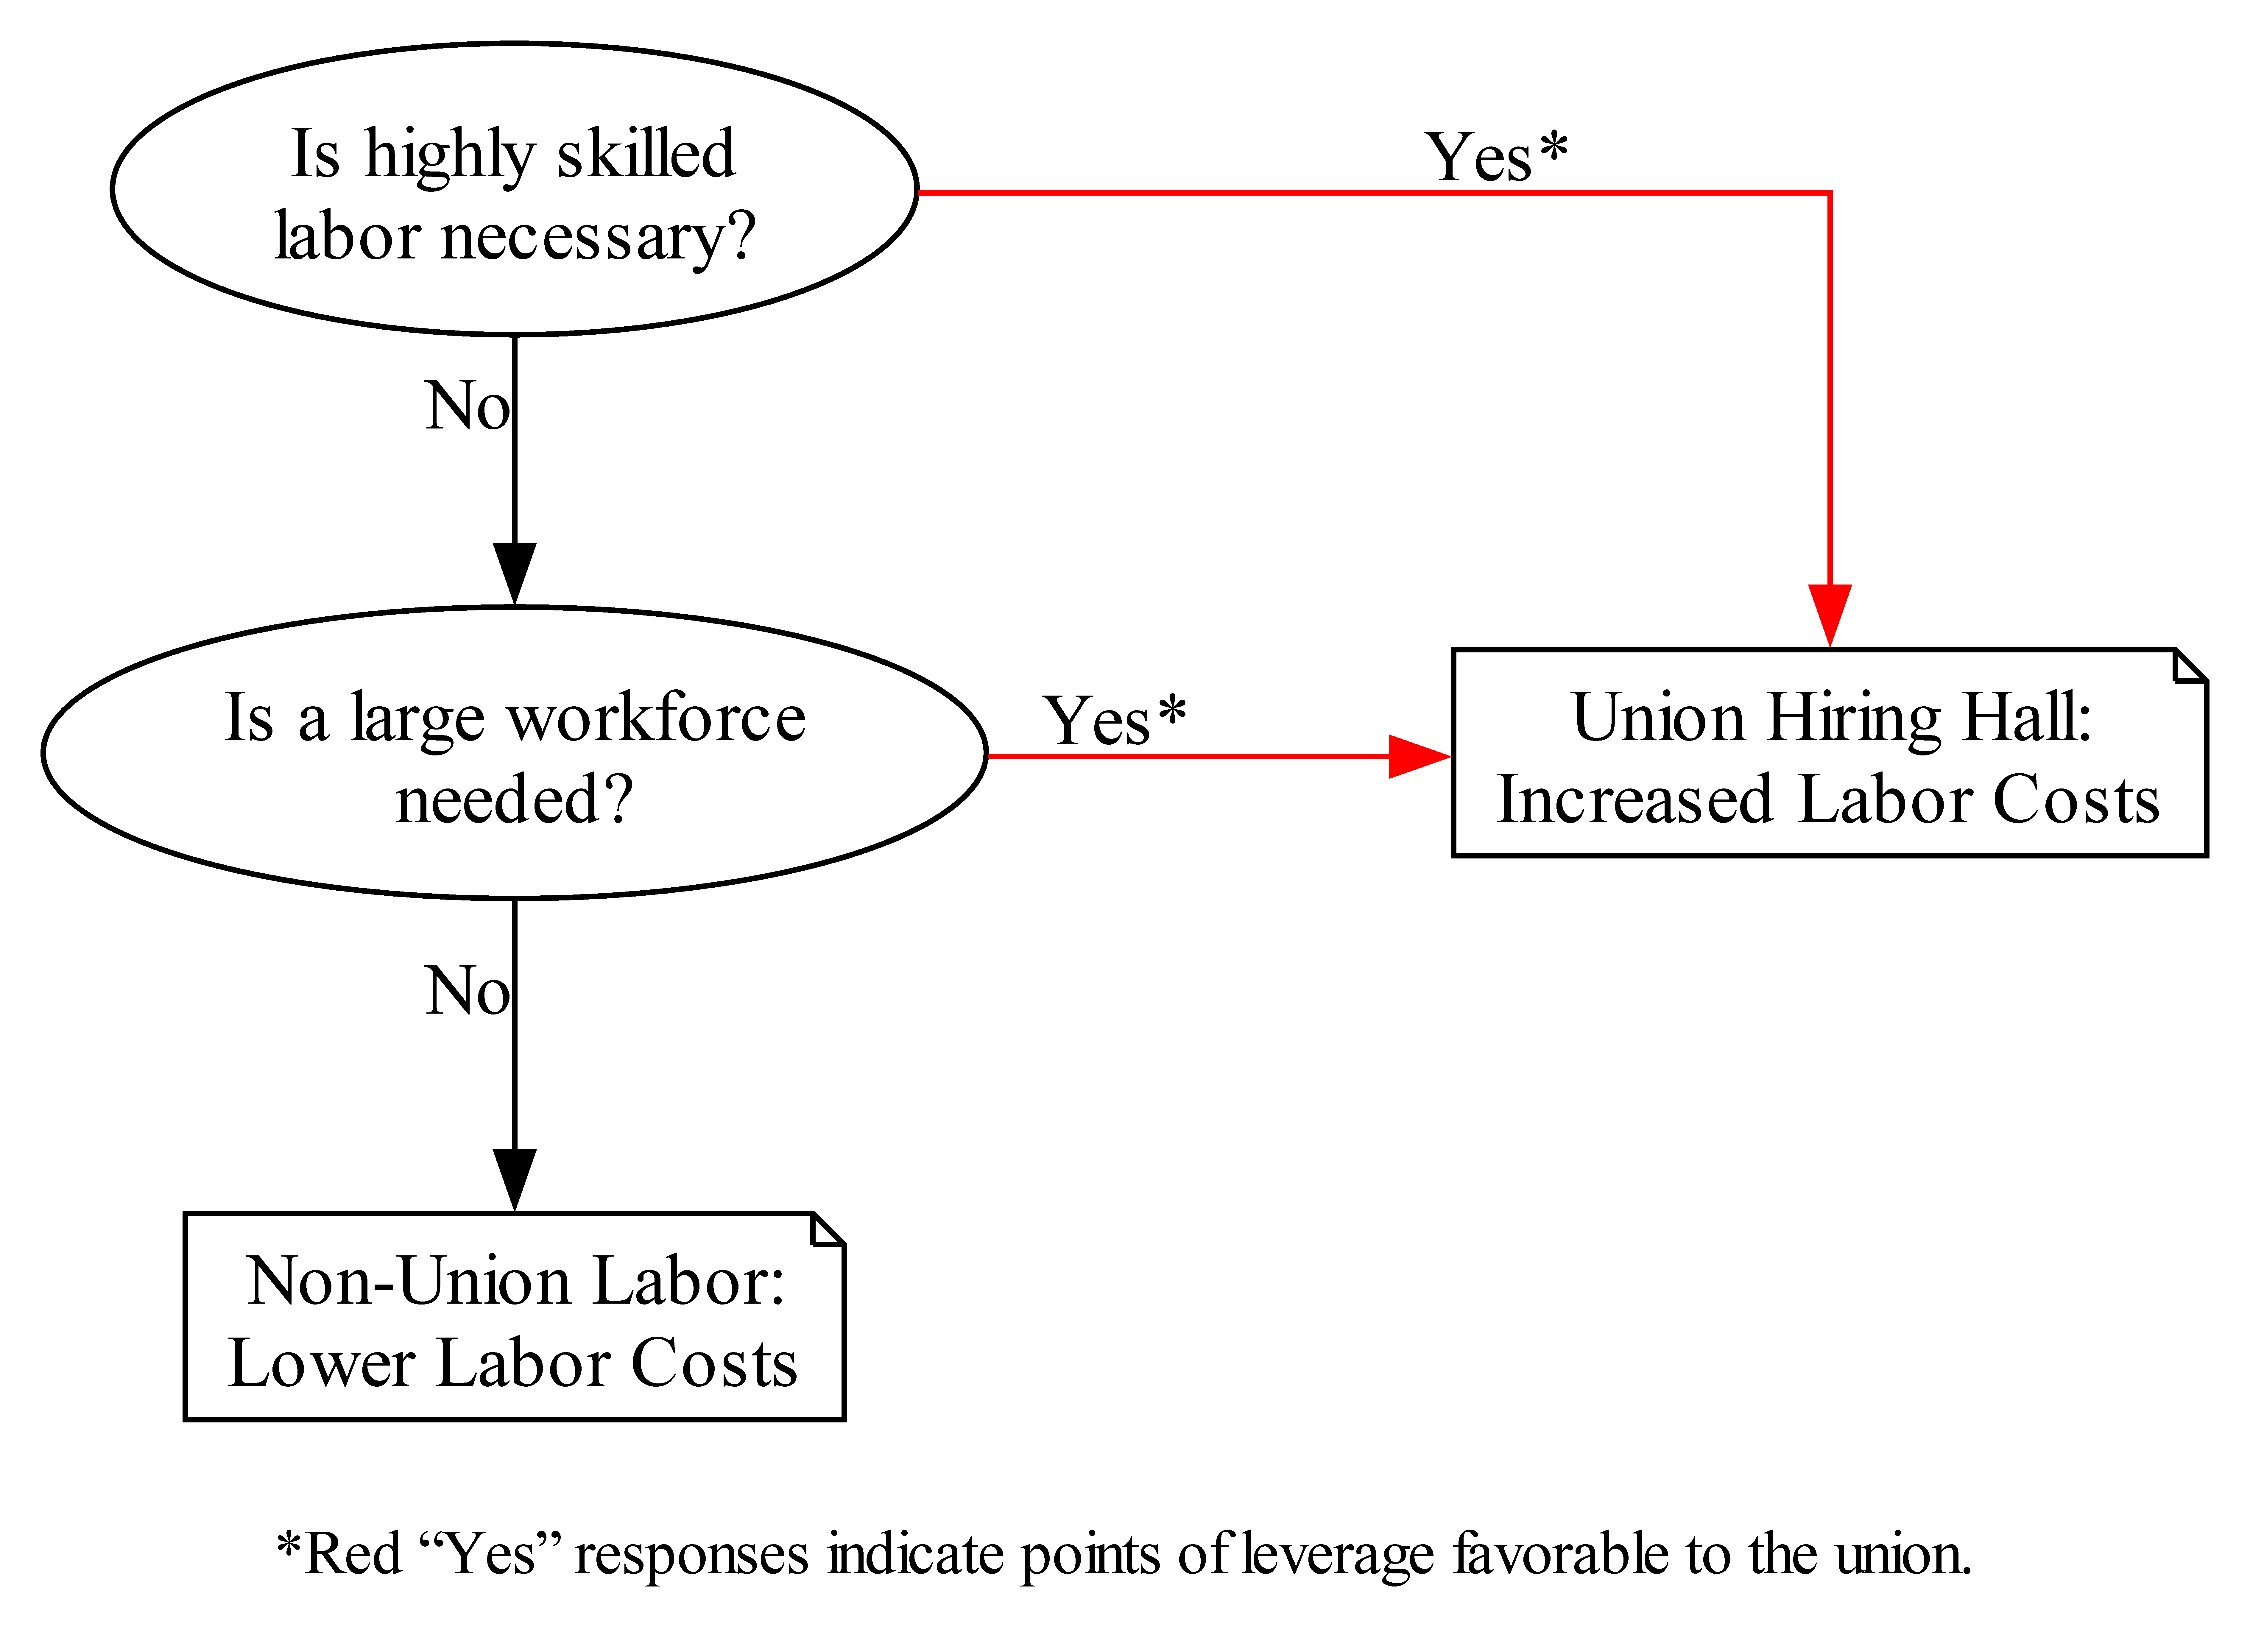
\includegraphics[width=\linewidth]{../images/union_power_red}

    \column{0.3\textwidth}
    Since negotiations between construction unions and employers are voluntary, construction unions typically have more leverage where the employer requires a more skilled workforce or where the job is large and requires many employees.
  \end{columns}
\end{frame}

\section{Conclusion}
\begin{frame}{Conclusion}
  This concludes my presentation.
\end{frame}

\end{document}
